
\subsection{Filter Functions}

\subsection{Topological Filtration}

\subsection{Topological Filtration of 1-D Simplicial Complexes}

% %%%%%%%%%%%%%%%%%%%%%%%%%%%%%%%%%%%%%%%%%%%%%%%%%%%%%%%%%
% PERSISTENCE DETAILS 
% WE ARENT DOING PERSISTENCE
% FILTRATION IS DIFFERENT THAN SIMPLIFICATION
% %%%%%%%%%%%%%%%%%%%%%%%%%%%%%%%%%%%%%%%%%%%%%%%%%%%%%%
\iffalse
%We begin by describing both the mathematical underpinnings and common computational tools for our topological data analysis.  Then, we review work on image segmentation and discuss how topological data analysis has started to be used in this context.  

% \subsection{Computational Topology}
% \label{bg:comp_topo}

%\paragraph{Topology in Segmentation}
%To alleviate the burden of manual segmentation, TDA has shown to be a useful and robust tool in aiding field experts for semantic feature extraction. Here, we present the relevant mathematical background that forms the underpinning of the Morse-Smale Complex (MSC), a powerful topological prior for image data analysis.  
%The use of TDA for easier and quicker segmentation by means of the 1-skeleton representation of the MSC has been seen across 
%Here, we present the relevant background to the Morse-Smale complex (MSC), the topological abstraction we use to generate ``priors'' objects for ML-assisted image segmentation. 
%%%%%%%%%%%%%%%%%%%%%%%%%%%%%%%%%%%%%%%%%%%%%%%%%%%%%%%%%
\subsection{The Morse-Smale Complex (MSC)}
\label{ssec:msc}
A Morse function $f: \mathcal{M}\rightarrow \mathbb{R}$ is a smooth function on a manifold with non-degenerate, distinct critical points. The gradient, $\nabla f$ defines a vector field whose zeroes are critical points. %{\it Integral lines} are paths tangent to $\nabla f$ with lower and upper limits at critical points of $f$. 
Each non-critical point in the domain of $\mathcal{M}$ belongs to a single integral line, or path tangent to $\nabla f$ that has upper and lower limits at critical points of $f$ (called the \emph{destination}, and \emph{origin}, respectively). The partitioning of the domain into monotonic connected components defined by integral lines sharing a common origin and destination defines the MSC. \textit{Cells} of this complex have a dimension equal to the difference between the number of source directions between the destination and origin critical points of their constituent integral lines. %Figure~\ref{mscbackground} (a, b) shows a scalar function and its corresponding MSC, and the relationships between cells.
The \textit{1-skeleton} of the complex is formed by critical points %, \textit{nodes}, 
and the \emph{arcs} or integral lines that connect them, where these differ in index by 1. 
% \begin{figure}[h!]
%  \centering
%  \resizebox{0.9\columnwidth}{!}{%
%  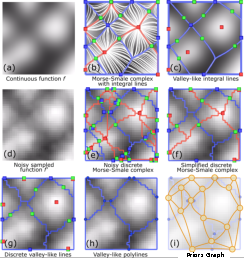
\includegraphics{./figures/mscbackground.pdf}
%  }
%      \caption{ Morse-Smale complexes are defined for functions with continuous gradients {\bf(a-c)}. A smooth function {\bf(a)} can be partitioned based on the behavior of integral lines {\bf(b)}, with selected integral lines shown in white. This partition forms a cell complex, where integral lines within each cell share a common origin and destination. The 0-dimensional cells are \red{maxima}, \green{saddles}, and \Blue{minima}), the 1-dimensional cells are formed by \dorange{ascending} and \lblue{descending lines} from \green{saddles}, and 2-dimensional cells are bounded by 0- and 1-cells {\bf(b)}. Elements of this complex often form semantic features of interest in a scientific domain, such as valley-like lines {\bf(c)}. Real-world functions often come from noisy sources, and are available as samples on a grid {\bf(d)}. Discrete Morse-theory-based methods allow practical computation of Morse-Smale complexes {\bf(e)}, which encode both noise and discretization artifacts that may be simplified to recover the coarse-scale behavior of the function {\bf(f)}. The valley-like structures may be extracted from this complex {\bf(g)}, and converted to a set of priors between non-degree-2 vertices denoted the valley graph {\bf(h)}. The \blonde{priors graph}, {\bf(i)}, represents each prior as a vertex with edges between incident priors. }
%      \label{mscbackground}
%  \end{figure}
%  
%\input{Background/msc_algorithm}
%\paragraph{Discrete Morse Theory}
%\label{sec:discrete-morse}
%The MSC is computed based on the gradient behavior of a continuous scalar function on a manifold. 
Concepts from continuous functions can be applied to a discrete pixel space using discrete Morse theory~\cite{formanMorse}, for which we use the open-source MSCEER library~\cite{MSCEER} to compute a discrete MSC complex. 

\vspace{-.3cm}

\subsection{Topological Simplification}
\label{ssec:pers}
Topological abstractions come equipped with well-understood techniques to order and simplify their elements to obtain successively coarser representations. For example, \textit{topological persistence} allows for a multiscale simplification by pairing the critical point that creates a connected component with the critical point that destroys that component during a filtration~\cite{edelsbrunner2000topological}. The time span in the filtration in which the connected component lives, \textit{i.e.} the difference in function value between the birth and death critical points, is called persistence. The admissible persistence defining this filtration defines the granularity of the resulting MSC~\cite{edelsbrunner2000topological, bremer2003, gyulassy2006topo}. 
% and similarly, the granularity of graphs in the persistence hierarchy. 
%To  
%This approach also affords a multiscale data structure defined by the simplification threshold, enabling a user to tune the simplification level and scale of the resulting complex to the data and task at hand.




 
 %The MSC 1-skeleton results from a multiscale simplification based on persistence in which pairs of critical points are removed upon the birth and death of topological features. Adjacent critical points adjoined by an integral line boundary, enclosing a region of uniform gradient, are removed, and their adjoining polyline reconnects with their respective neighboring critical points~\cite{gyulassy2006topo}. In image data analysis, often high-intensity elements correspond to ridge-like structures in a semantic object of interest. 

\fi
